
\section{Anforderungsspezifikation}
\label{Anforderungsspezifikation}

\subsection{Use Cases}
\label{Anforderungsspezifikation:Use Cases}

Im folgenden sind die funktionalen Anforderungen an das System mit all seinen Komponenten, welche im Kapitel \ref{Architektur} aufgeführt sind, als Use Cases im Brief-Format beschrieben.
Zur Übersicht ist das Use Case Diagramm in Abbildung \ref{fig:UseCase_OeV-Gueteklassen_2018} zu betrachten.

\begin{figure}[ht]
\centering
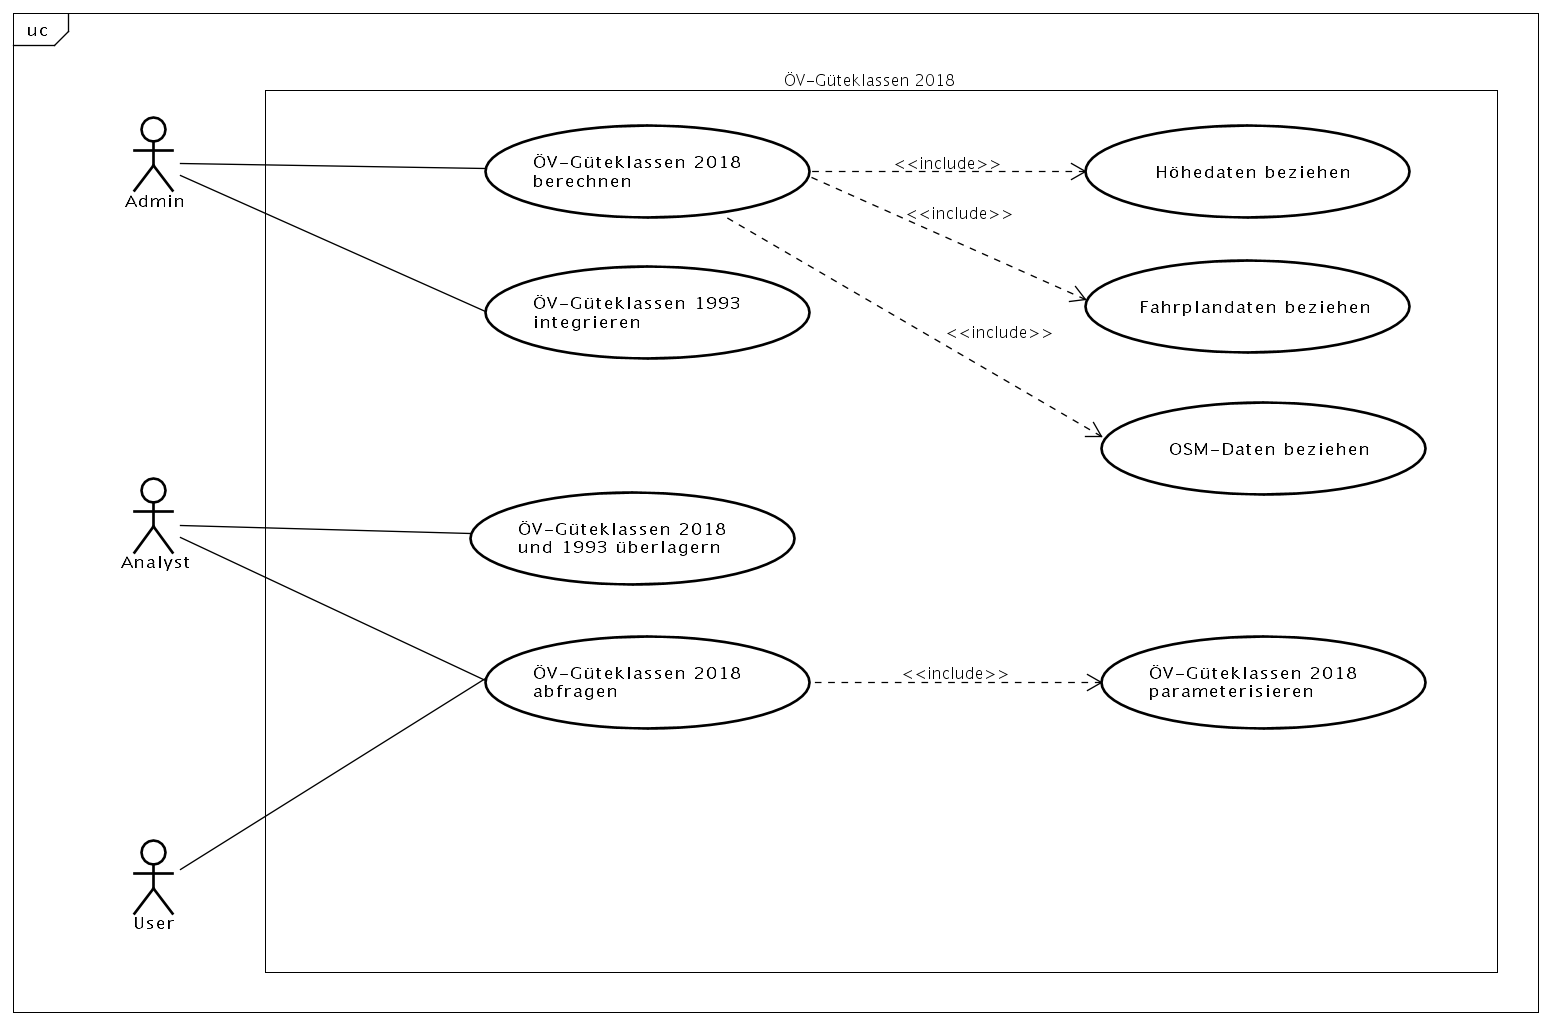
\includegraphics[width=1.0\linewidth]{projectdoc/img/UseCase_OeV-Gueteklassen_2018}
\caption[Use Case Diagramm]{Use Case Diagramm}
\label{fig:UseCase_OeV-Gueteklassen_2018}
\end{figure}

\subsubsection{Aktoren}
\label{Use Cases:Aktoren}

Um die Anforderungen akkurat evaluieren zu können, ist es essentiell, die Aktoren des Systems zu identifizieren.
In der Tabelle \ref{table:Aktoren} sind die Aktoren mit ihren Interessen aufgelistet.

\begin{longtable}{l p{14cm}}
        \toprule
        \textbf{Aktor}
                                & \textbf{Beschreibung und Interesse} \\
        \midrule
        \textbf{Admin}
                                & Ein \emph{Admin} ist für die Bereitstellung von akkuraten \acs{ÖV}-Güteklassen-Daten verantwortlich, welche er den Aktoren \emph{Analyst} und \emph{User} für die weitere Auswertung zur Verfügung stellt.
                                So möchte er die erforderlichen Daten sammeln und verarbeiten. \\
        \textbf{Analyst}
                                & Unter dem Aktor \emph{Analyst} sind Raum-/Verkehrsplaner, Transportgesellschaften und weitere Personen zusammengefasst, welche die \acs{ÖV}-Güteklassen-Daten für analytische Zwecke und als Planungsinstrument verwenden möchten. \\
        \textbf{User}
                                & Ein \emph{User} ist grundsätzlich am aktuellen Stand der \acs{ÖV}-Güteklassen in einer bestimmten Region interessiert, welche er als Basis für weitere Entscheidungen bezieht. \\
        \bottomrule
    \caption{Aktoren}
    \label{table:Aktoren}
\end{longtable}

\subsubsection{UC01: ÖV-Güteklassen 2018 berechnen}
\label{Use Cases:UC01}

Aktoren: \emph{Admin}

Include: \nameref{Use Cases:UC02}, \nameref{Use Cases:UC03}, \nameref{Use Cases:UC04}

Der \emph{Admin} startet die Berechnung der \acs{ÖV}-Güteklassen 2018 basierend auf einer Konfiguration (Stichtage und Zeitspannen) periodisch.


\subsubsection{UC02: Höhendaten vorverarbeiten}
\label{Use Cases:UC02}

Aktoren: \emph{Admin}

Der \emph{Admin} füḧrt das manuelle Beziehen der Höhendaten durch und übergibt diese dem System ''\acs{ÖV}-Güteklassen 2018''.
Das System bereit die Daten so vor, dass sie in \nameref{Use Cases:UC01} für die ''\acs{ÖV}-Güteklassen 2018''-Berechnung einbezogen werden können
Da die diese Daten nicht einem stetigen Wandel unterstehen, steht es dem \emph{Admin} frei, diesen Schritt auszulassen und bereits im System vorhandene, verarbeitete Höhendaten zu verwenden.

\subsubsection{UC03: Fahrplandaten periodisch vorverarbeiten}
\label{Use Cases:UC03}

Aktoren: \emph{Admin}

Der \emph{Admin} nutzt das System ''\acs{ÖV}-Güteklassen 2018'' für das periodische Beziehen der Fahrplandaten über eine externe Schnittstelle.
Das System bereit die Daten so vor, dass sie in \nameref{Use Cases:UC01} für die ''\acs{ÖV}-Güteklassen 2018''-Berechnung einbezogen werden können.

\subsubsection{UC04: OSM-Daten periodisch vorverarbeiten}
\label{Use Cases:UC04}

Aktoren: \emph{Admin}

Der \emph{Admin} nutzt das System ''\acs{ÖV}-Güteklassen 2018'' für das periodische Beziehen der \acs{OSM}-Daten über eine externe Schnittstelle.
Das System bereit die Daten so vor, dass sie in \nameref{Use Cases:UC01} für die ''\acs{ÖV}-Güteklassen 2018''-Berechnung einbezogen werden können.


\subsubsection{UC05: ÖV-Güteklassen 1993 integrieren}
\label{Use Cases:UC05}

Aktoren: \emph{Admin}

Der \emph{Admin} nutzt das System ''\acs{ÖV}-Güteklassen 2018'' für die Integration der ÖV-Güteklassen 1993.
% TODO hier ist mir noch nicht ganz klar, wie wir das machen. Analog zu 2018 einfach mit einer der bestehenden Berechnugsmethodik?

\subsubsection{UC06: ÖV-Güteklassen 2018 und 1993 vergleichen}
\label{Use Cases:UC06}

Aktoren: \emph{Analyst}

Der \emph{Analyst} nutzt das System ''\acs{ÖV}-Güteklassen 2018'' für den Vergleich der \acs{ÖV}-Güteklassen 1993 und 2018.
Das System präsentiert eine grafische Überlagerung der beiden \acs{ÖV}-Güteklassen.

\subsubsection{UC07: ÖV-Güteklassen 2018 abfragen}
\label{Use Cases:UC07}

Aktoren: \emph{Analyst, User}

Include: \nameref{Use Cases:UC08}

Die Aktoren \emph{Analyst} und \emph{User} nutzt das System ''\acs{ÖV}-Güteklassen 2018'', um die berechneten \acs{ÖV}-Güteklassen 2018 anzuzeigen.


\subsubsection{UC08: ÖV-Güteklassen 2018 parametrisieren}
\label{Use Cases:UC08}

Aktoren: \emph{Analyst, User}

Die Aktoren \emph{Analyst} und \emph{User} übergibt dem System ''\acs{ÖV}-Güteklassen 2018'' eine Konfiguration der anzuzeigenden \acs{ÖV}-Güteklassen 2018.
Das System ''\acs{ÖV}-Güteklassen 2018'' liefert auf Basis dieser die zugehörigen, vorgerechneten Daten.

\subsection{Nicht-funktionale Anforderungen}
\label{Anforderungsspezifikation:Nicht-funktionale Anforderungen}

\subsubsection{NFA01: TODO}
\label{NFA:NFA01}

%TODO

